\documentclass{beamer}
\usepackage{array}
\usepackage{graphicx}
\usetheme{Madrid}

% Suppress the navigation bar and remove name and date from slides
\setbeamertemplate{navigation symbols}{}
\setbeamertemplate{footline}{}  % Removes the footer line with the author and date
\setbeamertemplate{headline}{}  % Removes the header line

% Title page details
\title{Conversational Used Car Price Predictor}
\subtitle{CS702 - Computing Lab}
\author{ABHIJITH C \and ANAND M K}
\institute{Department of Computer Science and Engineering \\ NITK Surathkal}
\date{}  % No date on title slide

\begin{document}

% Title page
\begin{frame}[t]
    \titlepage
\end{frame}

% Slide 1: Introduction
\begin{frame}[t]{Introduction}
    \begin{columns}
        \column{0.6\textwidth}
        \begin{itemize}
            \item Conversational interfaces enhance interaction with technology.
            \item The used car market is growing, and accurate price evaluation can be challenging.
            \item Machine learning helps predict car prices by analyzing various parameters.
            \item Goal: Develop a conversational interface to predict used car prices.
        \end{itemize}
        
        \column{0.4\textwidth}
        \centering
        
\includegraphics[width=\linewidth]{Chatbot.jpg}  % Replace 'your_image.png' with your image file
    \end{columns}
\end{frame}

% Slide 2: Problem Statement and Objectives
\begin{frame}[t]{Problem Statement and Objectives}
    \begin{columns}
        \column{0.6\textwidth}
        \begin{itemize}
        \item Predicting used car prices requires multiple parameters such as manufacturer, model, year, mileage, etc.
        \item Traditional methods are often less interactive and user-friendly.
        \item This project aims to develop a chatbot integrated with a price prediction model for a more intuitive user experience.
        \end{itemize}
        
        \column{0.4\textwidth}
        \centering
        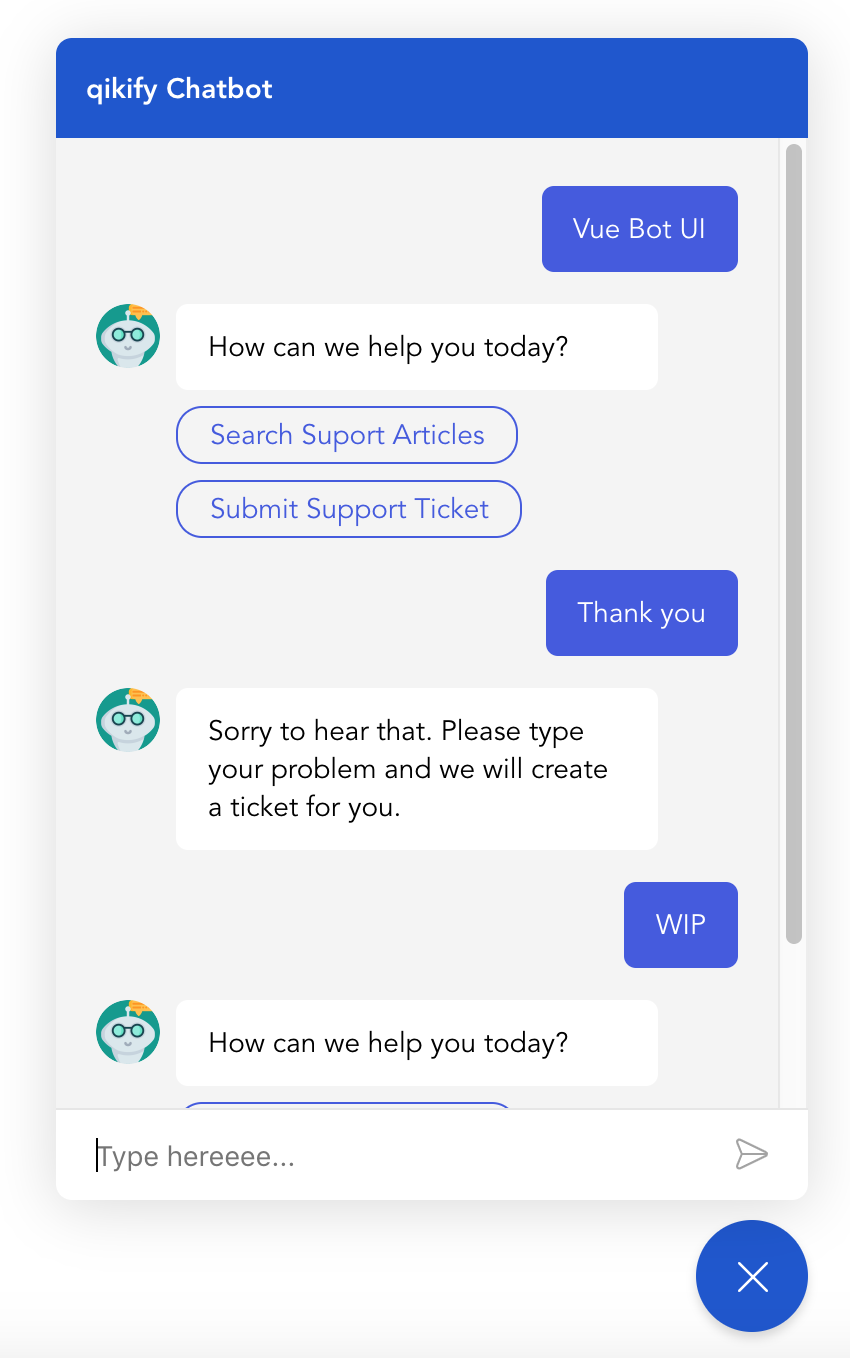
\includegraphics[width=\linewidth]{interface.png}  % Replace 'your_image.png' with your image file
    \end{columns}
\end{frame}

% Slide: Literature Survey with Table
\begin{frame}[t]{Literature Survey}
    \small % Reduce font size for table content
    \resizebox{\textwidth}{!}{  % Rescale the table to fit the slide
    \begin{tabular}{|c|m{4cm}|c|m{5cm}|}
        \hline
        \textbf{S.No.} & \textbf{Title} & \textbf{Year} & \textbf{Methodology} \\ \hline
        1 & Prediction of Used Car Prices Using Artificial Neural Networks & 2022 & Artificial Neural Networks (ANN) for price prediction \\ \hline
        2 & Conversational AI Unleashed: A Comprehensive Review of NLP-Powered Chatbot Platforms & 2023 & NLP-powered chatbot platform for natural language interaction \\ \hline
        3 & Predicting the Sale Price of Pre-Owned Vehicles with the Ensemble ML Model & 2023 & Ensemble methods using Random Forest for price prediction \\ \hline
        4 & Challenges and Solutions in Conversational AI & 2017 & End-to-end conversational AI architecture \\ \hline
        5 & Improving User Experience in Conversational Systems & 2018 & Enhancing chatbot systems with personalized responses \\ \hline
    \end{tabular}
    }
\end{frame}

\begin{frame}[t]{Proposed Methodology}
    \begin{itemize}
        \item Conduct requirement analysis to identify user needs and key functionalities.
        \item Design the dialogue flow, defining user intents and entities for intuitive interactions.
        \item Implement Natural Language Processing (NLP) libraries to process user input.
        \item Generate appropriate responses based on user queries.
    \end{itemize}
\end{frame}




% Continue with the rest of the content (solution, phases, expected outcomes, etc.)
% ...

\end{document}
